\subsubsection{Crustal deformation}
\label{sec:cookbooks-crustal-deformation}

\textit{This section was contributed by Cedric Thieulot, and makes use of the Drucker-Prager
material model written by Anne Glerum and the free surface plugin by Ian Rose.}

This is a simple example of an upper-crust undergoing compression or extension.
It is characterized by a single layer of visco-plastic material subjected to basal
kinematic boundary conditions. In compression, this setup is somewhat analogous
to \cite{will99}, and in extension to \cite{alht11}.

Brittle failure is approximated by adapting the viscosity to limit the stress
that is generated during deformation.
This ``cap'' on the stress level is parameterized in this experiment by the pressure-dependent
Drucker Prager yield criterion  and we therefore make use of the Drucker-Prager
material model (see Section \ref{parameters:Material_20model}) in the
{\tt cookbooks/crustal\_deformation/crustal\_model\_2D.prm}.

The layer is assumed to have dimensions of $\SI{80}{km} \times \SI{16}{km}$ and to have a density  $\rho=\SI{2800}{kg/m^3}$.
The plasticity parameters are specified as follows:

\lstinputlisting[language=prmfile]{cookbooks/crustal_deformation/doc/crustal_model_2D_part1.prm.out}

The yield strength $\sigma_y$ is a function of pressure, cohesion and angle of friction
(see Drucker-Prager material model in Section \ref{parameters:Material_20model}),
and the effective viscosity is then computed as follows:
\[
\mu_{\text{eff}} = \left( \frac{1}{ \frac{\sigma_y}{2 \dot{\epsilon}}+
\mu_{\text{min}}} + \frac{1}{\mu_{\text{max}}}  \right)^{-1}
\]
where $\dot{\epsilon}$ is the square root of the second invariant of the deviatoric strain rate.
The viscosity cutoffs ensure that the viscosity remains within computationally acceptable values.

During the first iteration of the first timestep, the strain rate is zero, so
we avoid dividing by zero by setting the strain rate to {\tt Reference strain rate}.


The top boundary is a free surface while the left, right and bottom boundaries are subjected
to the following boundary conditions:

\lstinputlisting[language=prmfile]{cookbooks/crustal_deformation/doc/crustal_model_2D_part2.prm.out}

Note that compressive boundary conditions are simply achieved by reversing
the sign of the imposed velocity.

The free surface will be advected up and down according to the solution of the Stokes solve.
We have a choice whether to advect the free surface in the direction of the surface normal
or in the direction of the local vertical (i.e., in the direction of gravity).
For small deformations, these directions are almost the same, but in this example the deformations
are quite large. We have found that when the deformation is large, advecting the surface vertically
results in a better behaved mesh, so we set the following in the free surface subsection:

\lstinputlisting[language=prmfile]{cookbooks/crustal_deformation/doc/crustal_model_2D_part3.prm.out}

We also make use of the strain rate-based mesh refinement plugin:

\lstinputlisting[language=prmfile]{cookbooks/crustal_deformation/doc/crustal_model_2D_part4.prm.out}

Setting
{\tt   set Initial adaptive refinement        = 4}
yields a series of meshes as shown in Fig. (\ref{fig:meshes}), all produced during the
first timestep. As expected, we see that the location of the highest mesh refinement
corresponds to the location of a set of conjugated shear bands.

If we now set this parameter to 1 and allow the simulation to evolve
for 500kyr, a central graben or plateau (depending on the nature
of the boundary conditions) develops and deepens/thickens over time, nicely showcasing
the unique capabilities of the code to handle free surface large deformation, localised
strain rates through visco-plasticity and adaptive mesh refinement as
shown in Fig. (\ref{fig:extcompr}).

\begin{figure}
   \centering
   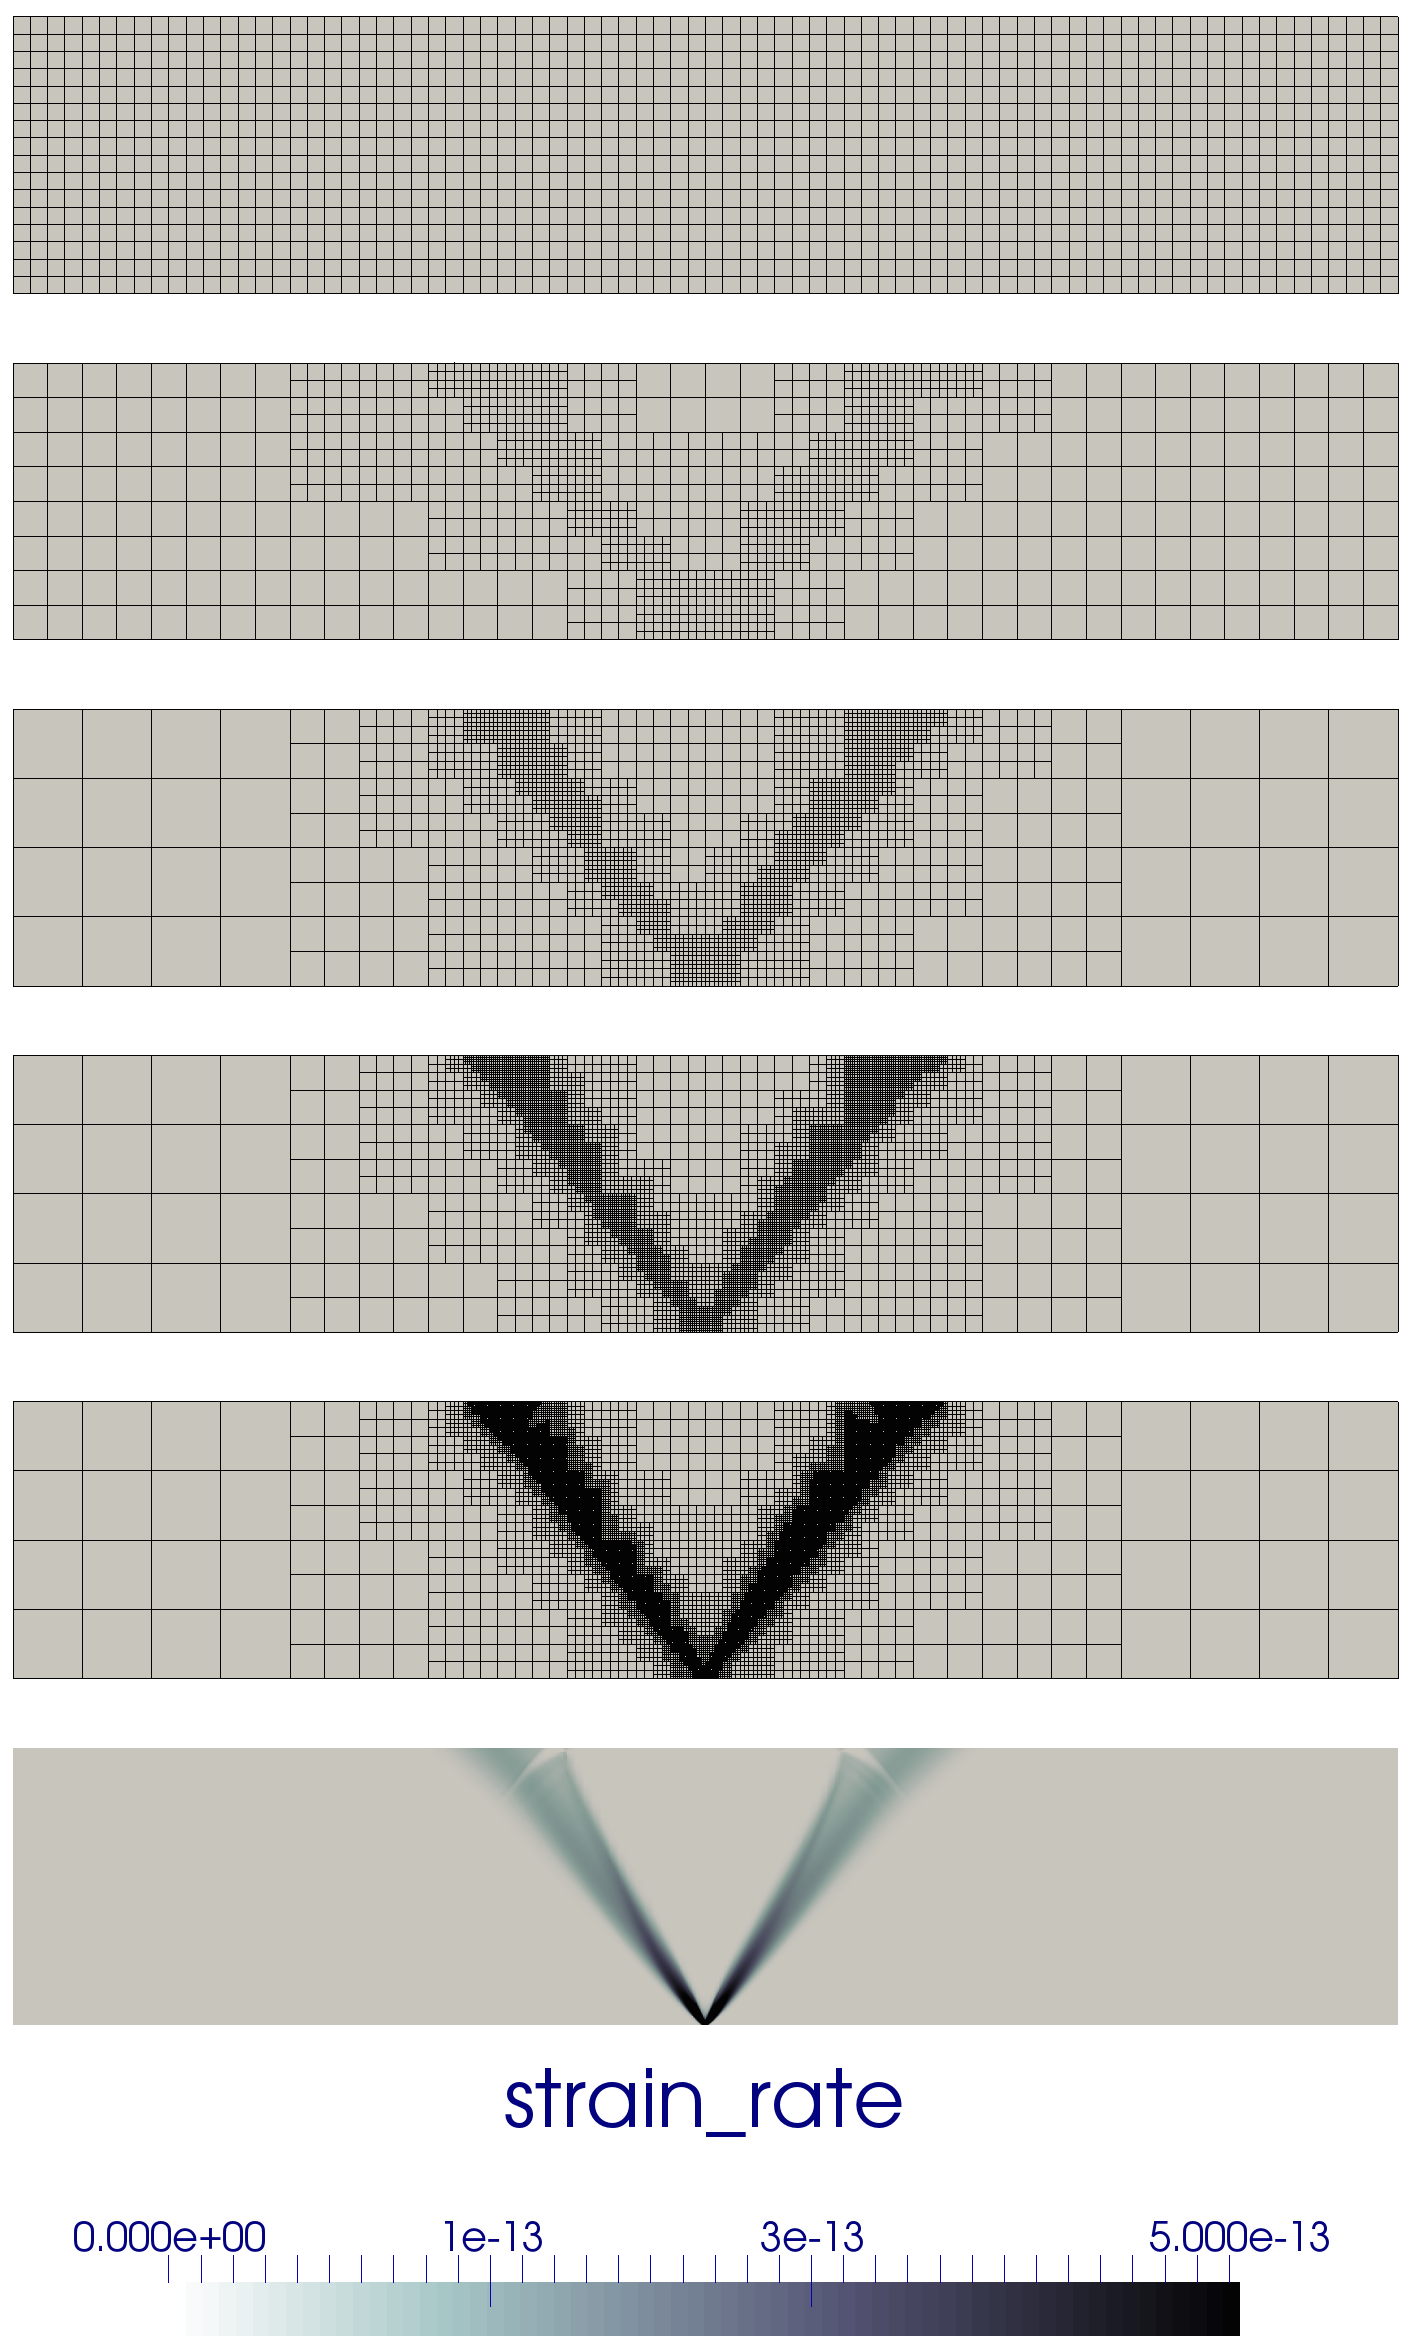
\includegraphics[width=0.7\textwidth]{cookbooks/crustal_deformation/doc/grids.png}
   \caption{\it Mesh evolution during the first timestep (refinement is based on strain rate).}
   \label{fig:meshes}
\end{figure}



Deformation localizes at the basal velocity discontinuity and plastic shear bands
form at an angle of approximately $53\degree$ to the bottom in extension and
$35\degree$ in compression, both of which correspond to the reported Arthur angle \cite{kaus10,buit12}.

\begin{figure}
  \centering
  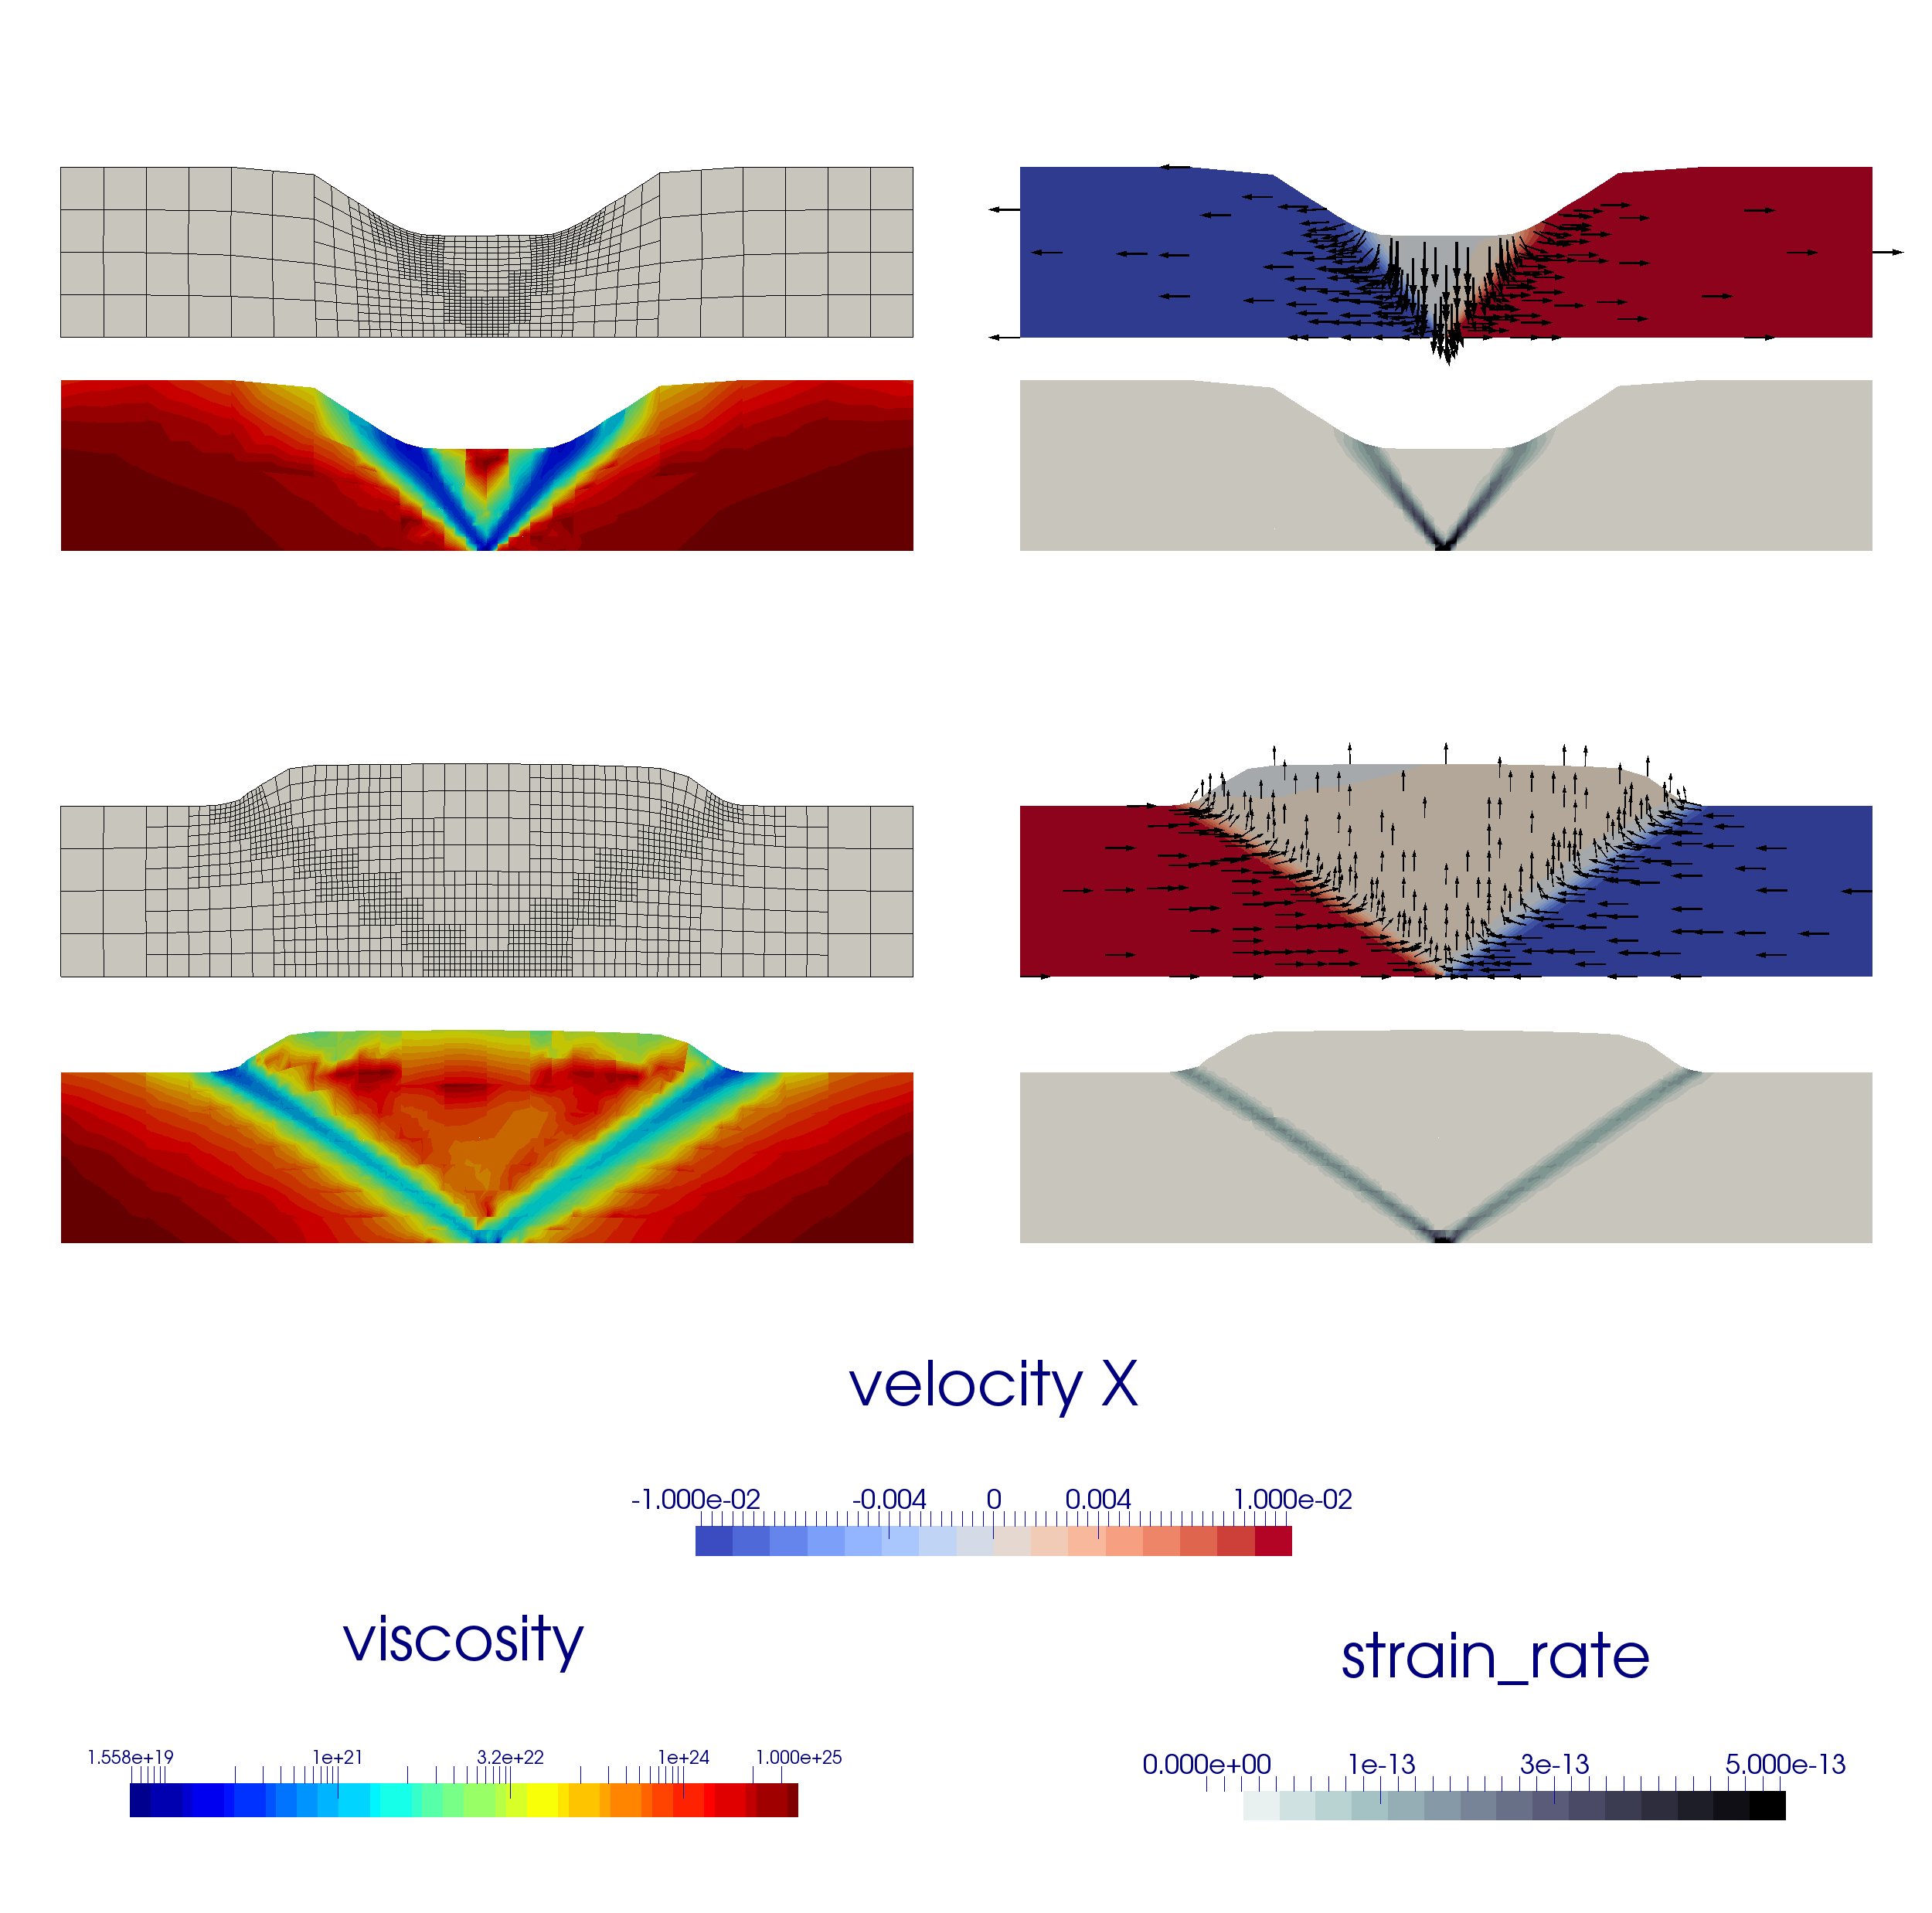
\includegraphics[width=\textwidth]{cookbooks/crustal_deformation/doc/both.png}
  \caption{\it Finite element mesh, velocity, viscosity and strain rate fields
  in the case of extensional boundary conditions (top) and compressive boundary conditions (bottom) at t=500kyr.}
  \label{fig:extcompr}
\end{figure}



\paragraph{Extension to 3D.} We can easily modify the previous
input file to produce {\tt crustal\_model\_3D.prm}
which implements a similar setup, with the additional constraint that the position
of the velocity discontinuity varies with the $y$-coordinate,
as shown in Fig. (\ref{fig:bottombc}).
The domain is now
$128\times96\times16$km and the boundary conditions are implemented as
follows:

\lstinputlisting[language=prmfile]{cookbooks/crustal_deformation/doc/crustal_model_3D_part1.prm.out}

The presence of
an offset between the two velocity discontinuity zones leads to a transform
fault which connects them.

\begin{figure}
  \centering
  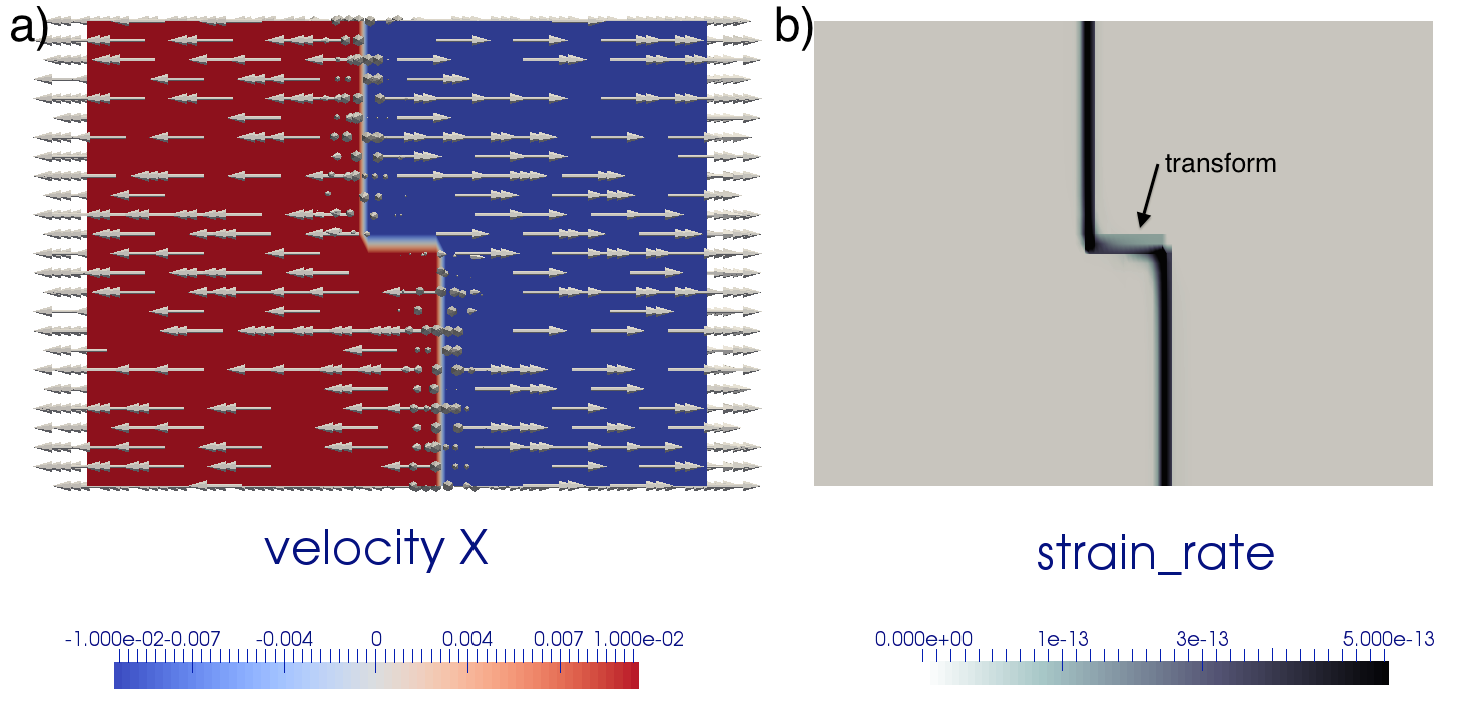
\includegraphics[width=\textwidth]{cookbooks/crustal_deformation/doc/bottombc2.png}
  \caption{\it Basal velocity boundary conditions and corresponding
  strain rate field for the 3D model.}
  \label{fig:bottombc}
\end{figure}

The Finite Element mesh, the velocity, viscosity and strain rate fields are shown
in Fig. (\ref{fig:ext3D}) at the end of the first time steps. The reader is encouraged
to run this setup in time to look at how the two grabens interact as a function
of their initial offset \cite{alht11,alht12,alhf13}.

\begin{figure}
\centering
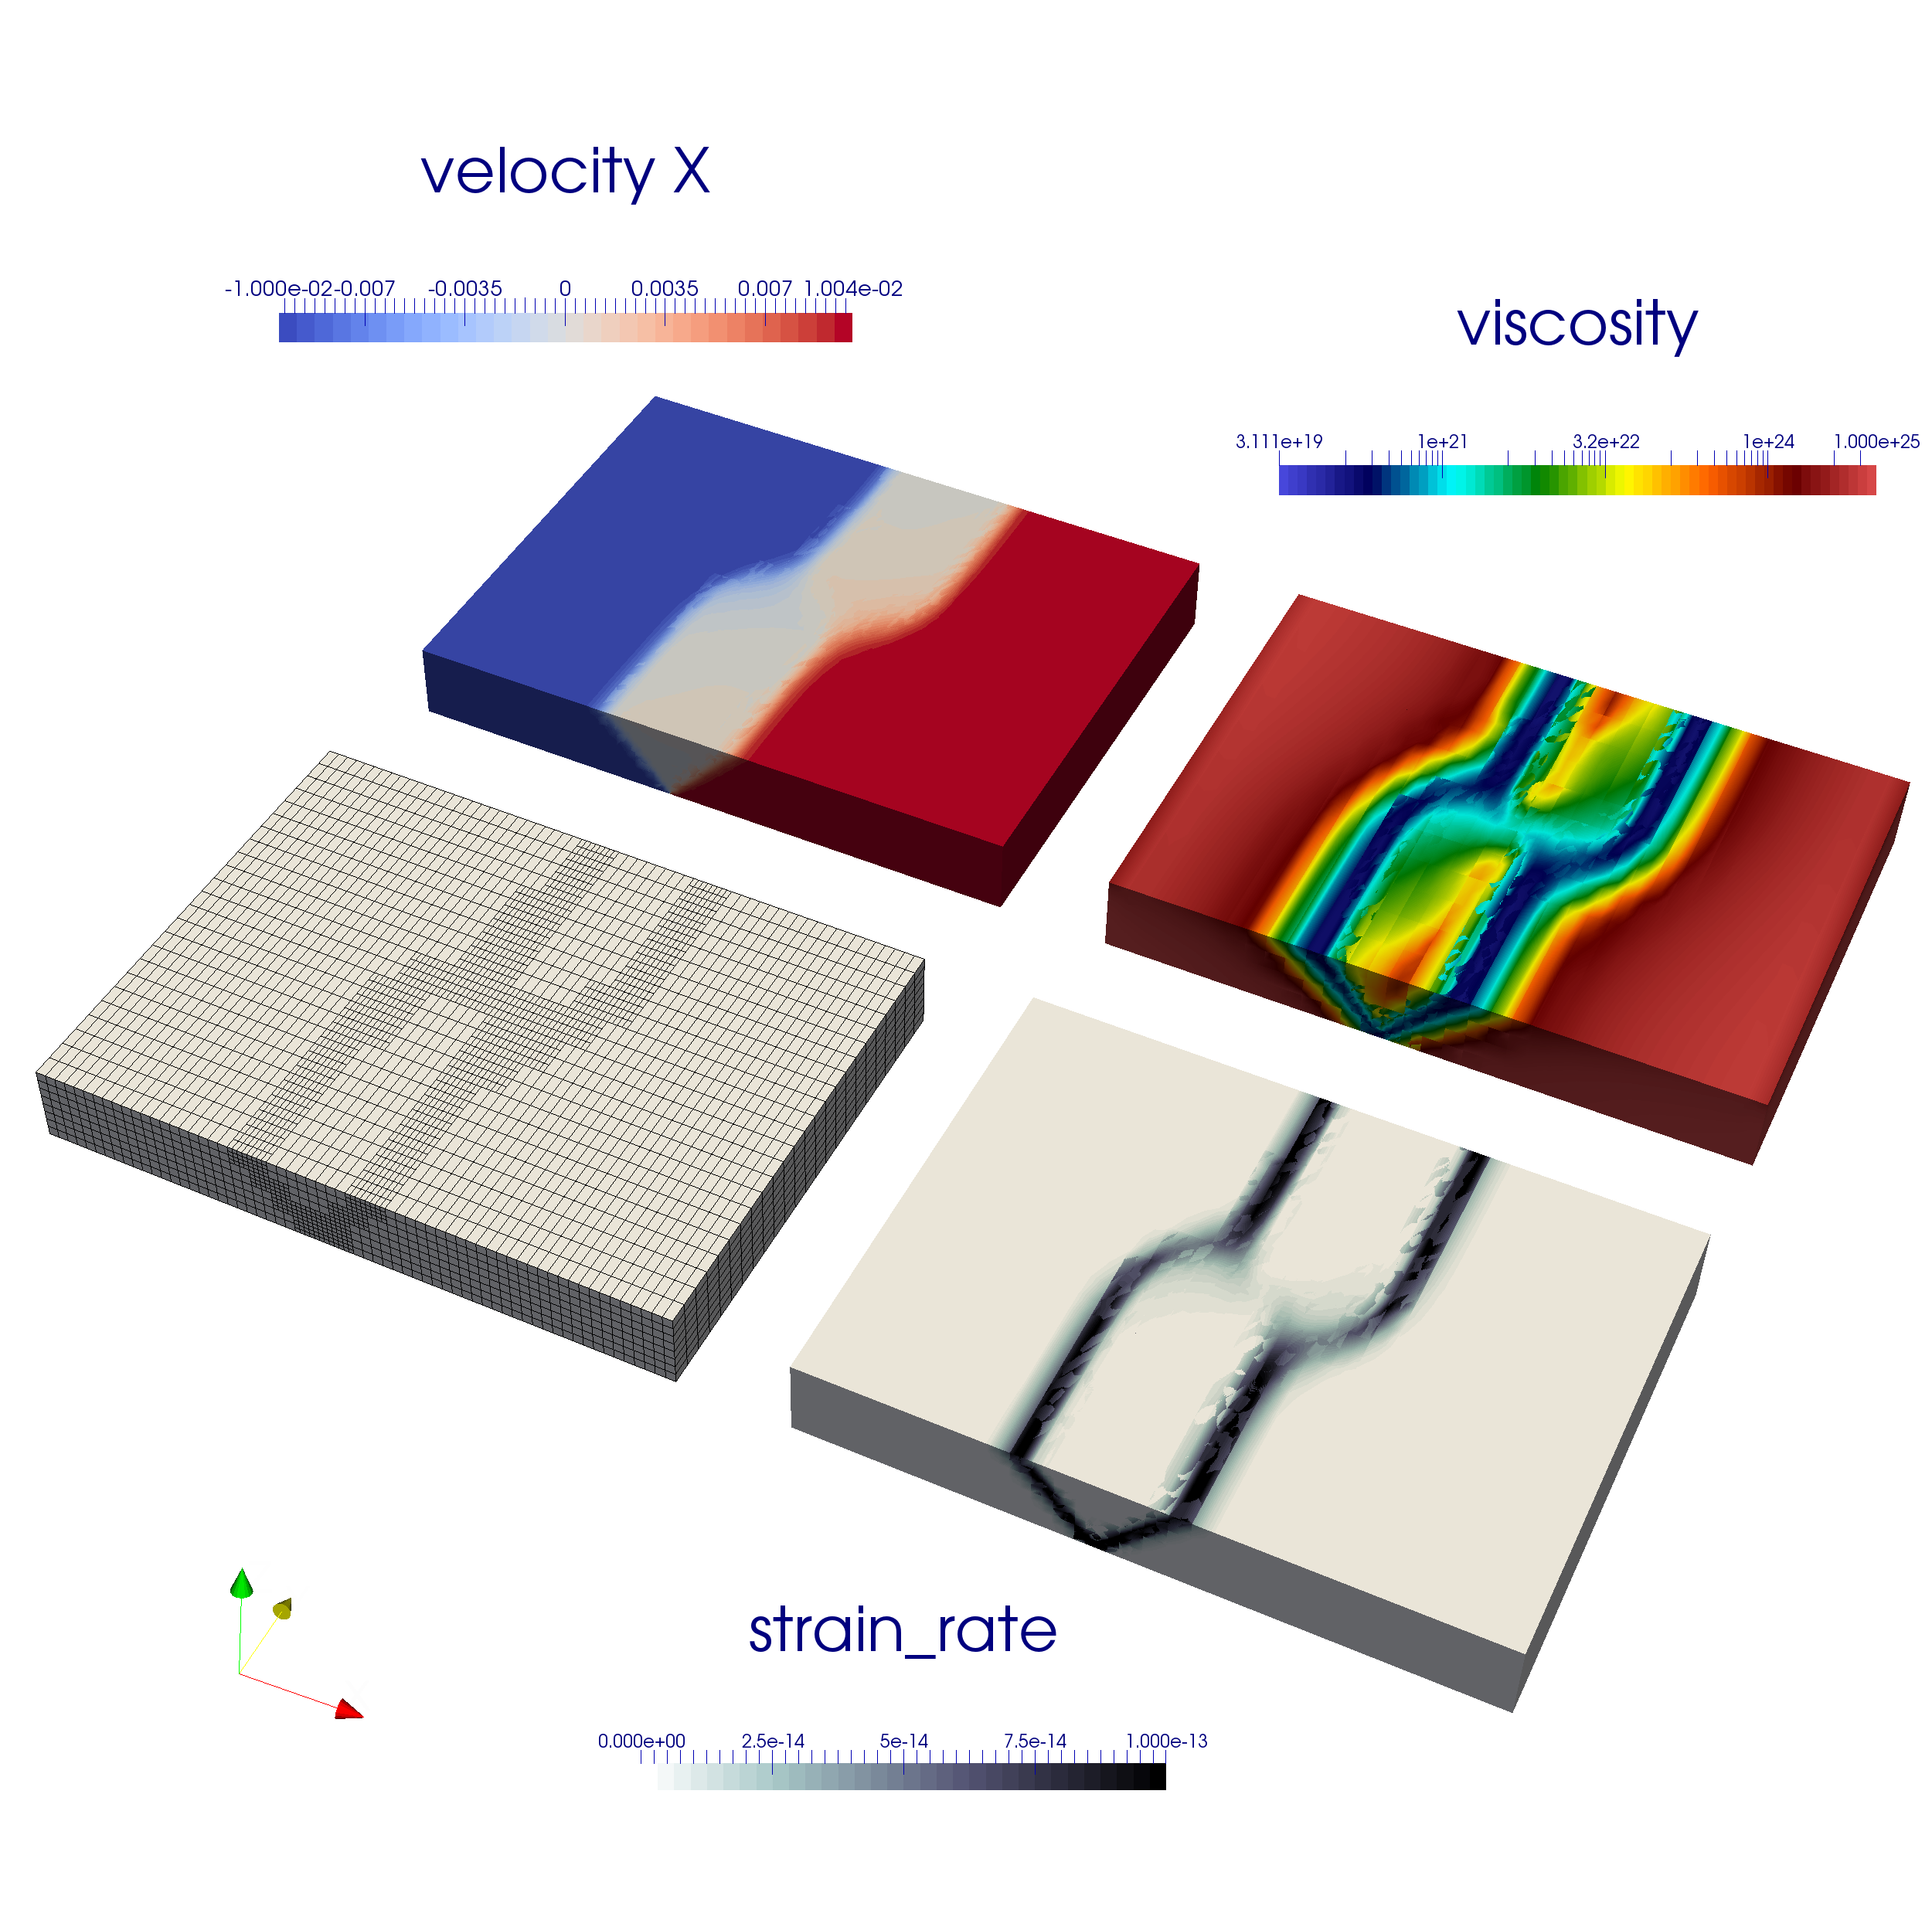
\includegraphics[width=\textwidth]{cookbooks/crustal_deformation/doc/all3D.png}
\caption{\it Finite element mesh, velocity, viscosity and strain rate fields at
the end of the first time step after one level of strain rate-based adaptive mesh refinement.}
\label{fig:ext3D}
\end{figure}
